\chapter{Pruebas de funcionalidad}\label{chapter:implementation}
En este capítulo se realizan un conjunto de pruebas para demostrar el buen funcionamiento de las herramientas implementadas y así evidenciar el cumplimiento de los
objetivos planteados en este trabajo.
Las pruebas se realizaron en dos dispositivos Android físicos y uno emulado desde Android Studio para abarcar la mayor cantidad de casos posibles\\
Los dispositivos tienen las siguientes prestaciones:\\
\section{Prestaciones de los dispositivos sobre los que se ejecutaron las pruebas}
\subsection{LG VELVET Android 13 [Dispositivo físico]}
\begin{itemize}
    \item 5.7 Gb RAM
    \item CPU Octa-Core a una frecuencia promedio por núcleo de 1.925 GHz
\end{itemize}
\subsection{Samsung Galaxy S23 Ultra Android 14 [Dispositivo físico]}
\begin{itemize}
    \item 8.0 Gb RAM
    \item CPU Octa-Core a una frecuencia promedio por núcleo de 2.57 GHz
\end{itemize}

\subsection{Google Pixel 4 Android 10 [emulador]}
\begin{itemize}
    \item 2.0 Gb RAM
    \item CPU Quad-Core
\end{itemize}


\section{Importación de un mapa}
En esta prueba se intenta importar un mapa en la aplicación tanto haciendo uso del botón con esta funcionalidad ubicado en la ventana que se muestra al
presionar el botón con icono de archivo en la esquina superior derecha de la aplicación; como también copiando el mapa de manera manual
hacia la carpeta "$ $CADIC/Maps"$ $ ubicada en el directorio raíz del dispositivo. Al importar el mapa como archivo con extensión '.mbtiles' este debería
aparecer en el área central al estar activa la pestaña 'Mapa'. En la figura \ref{fig:figura20} se aprecian los resultados.
\begin{figure}[h]
    % \centering
    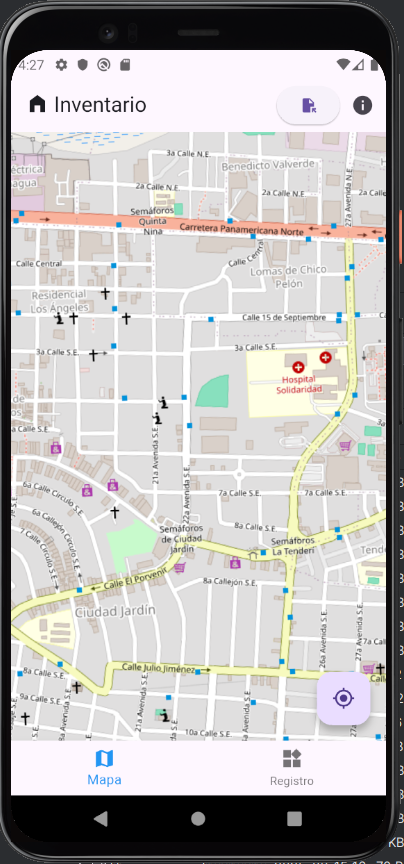
\includegraphics[width=0.3\textwidth]{Graphics/Capitulo 4/Pixel 4 [emulador]/4.2/1.png}
    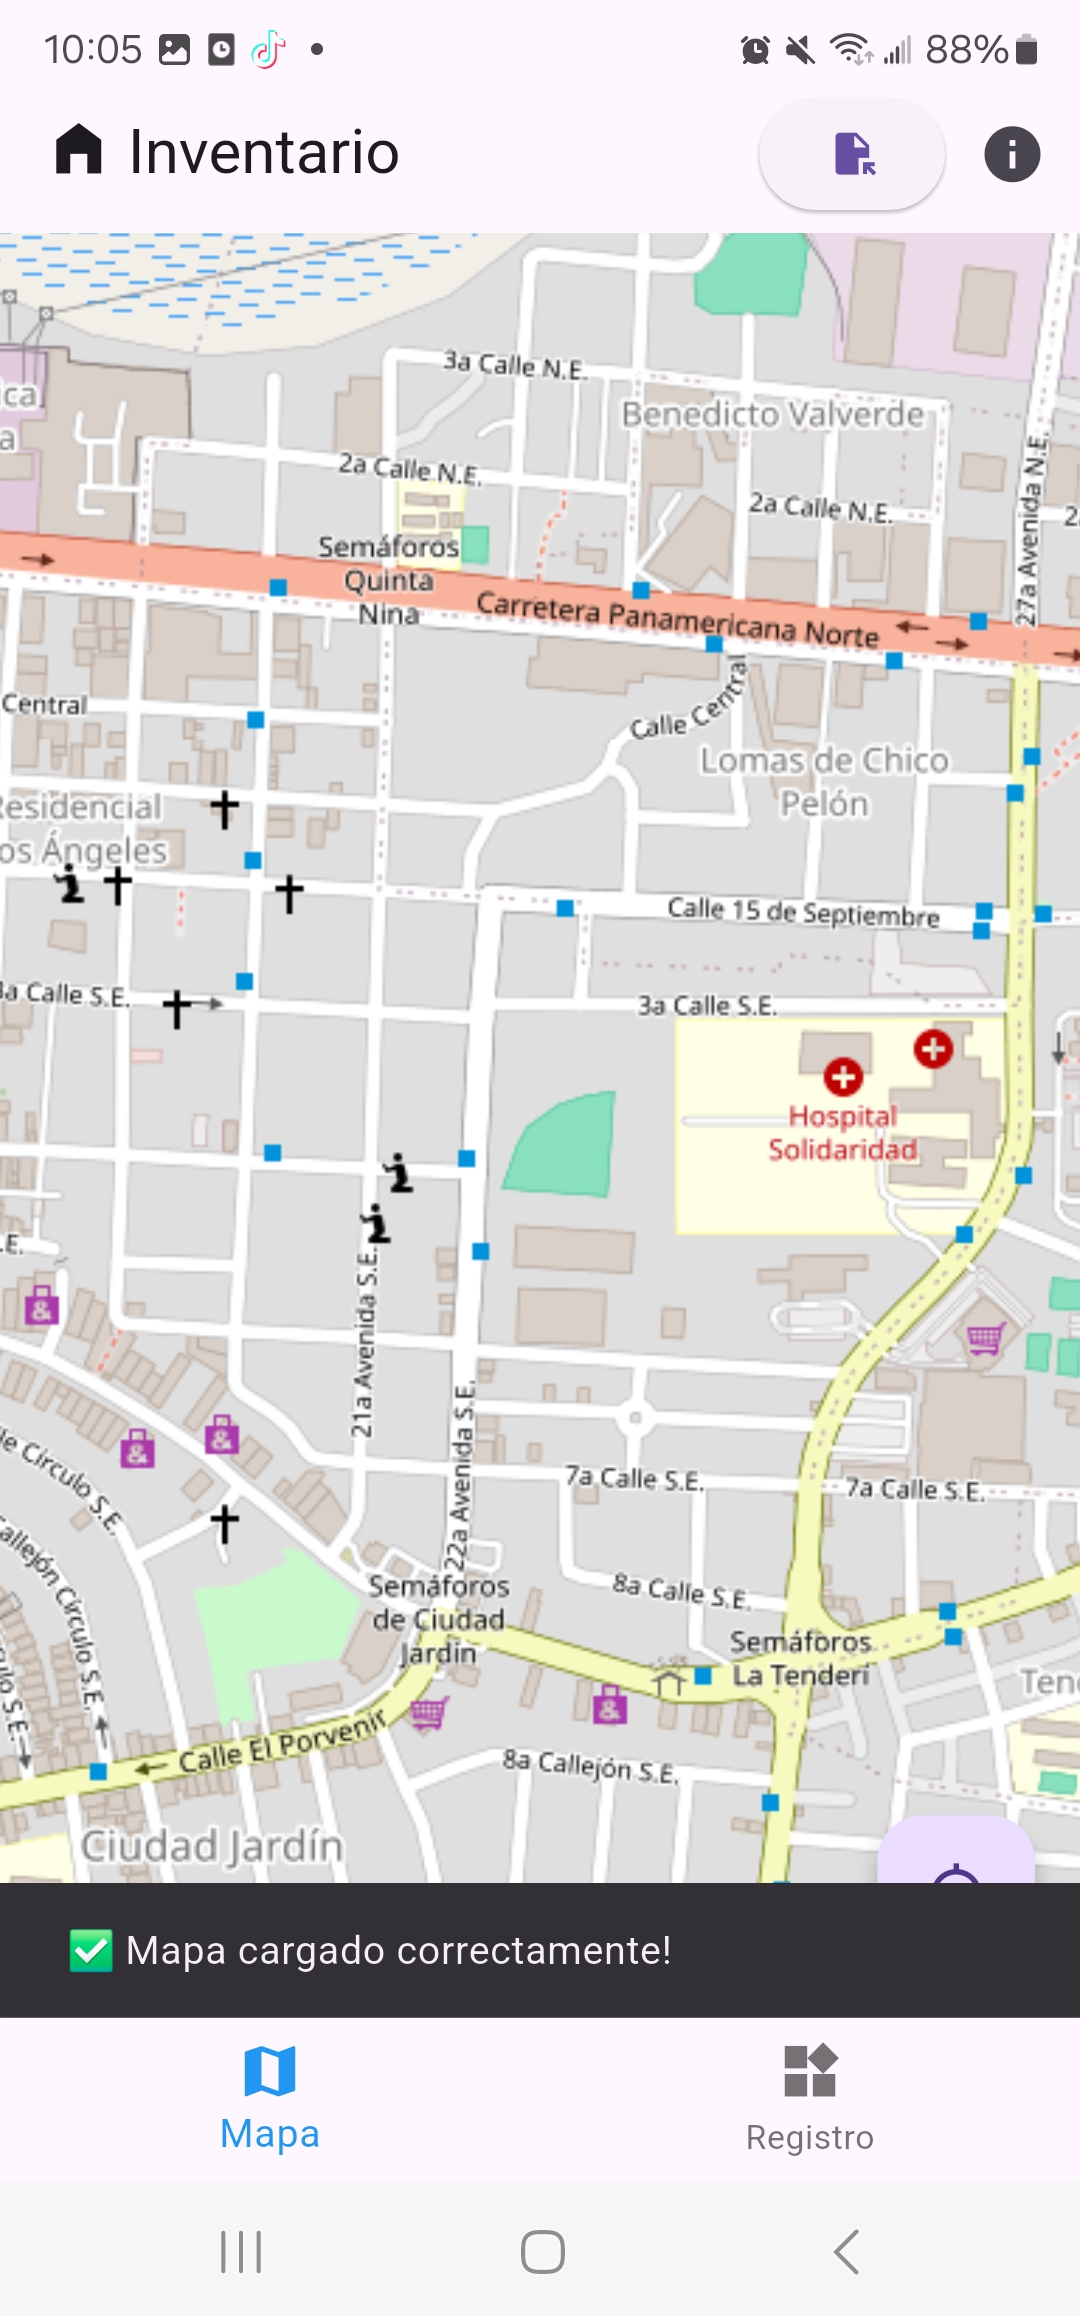
\includegraphics[width=0.3\textwidth]{Graphics/Capitulo 4/Galaxy S23 Ultra Android/4.2/3.jpg}
    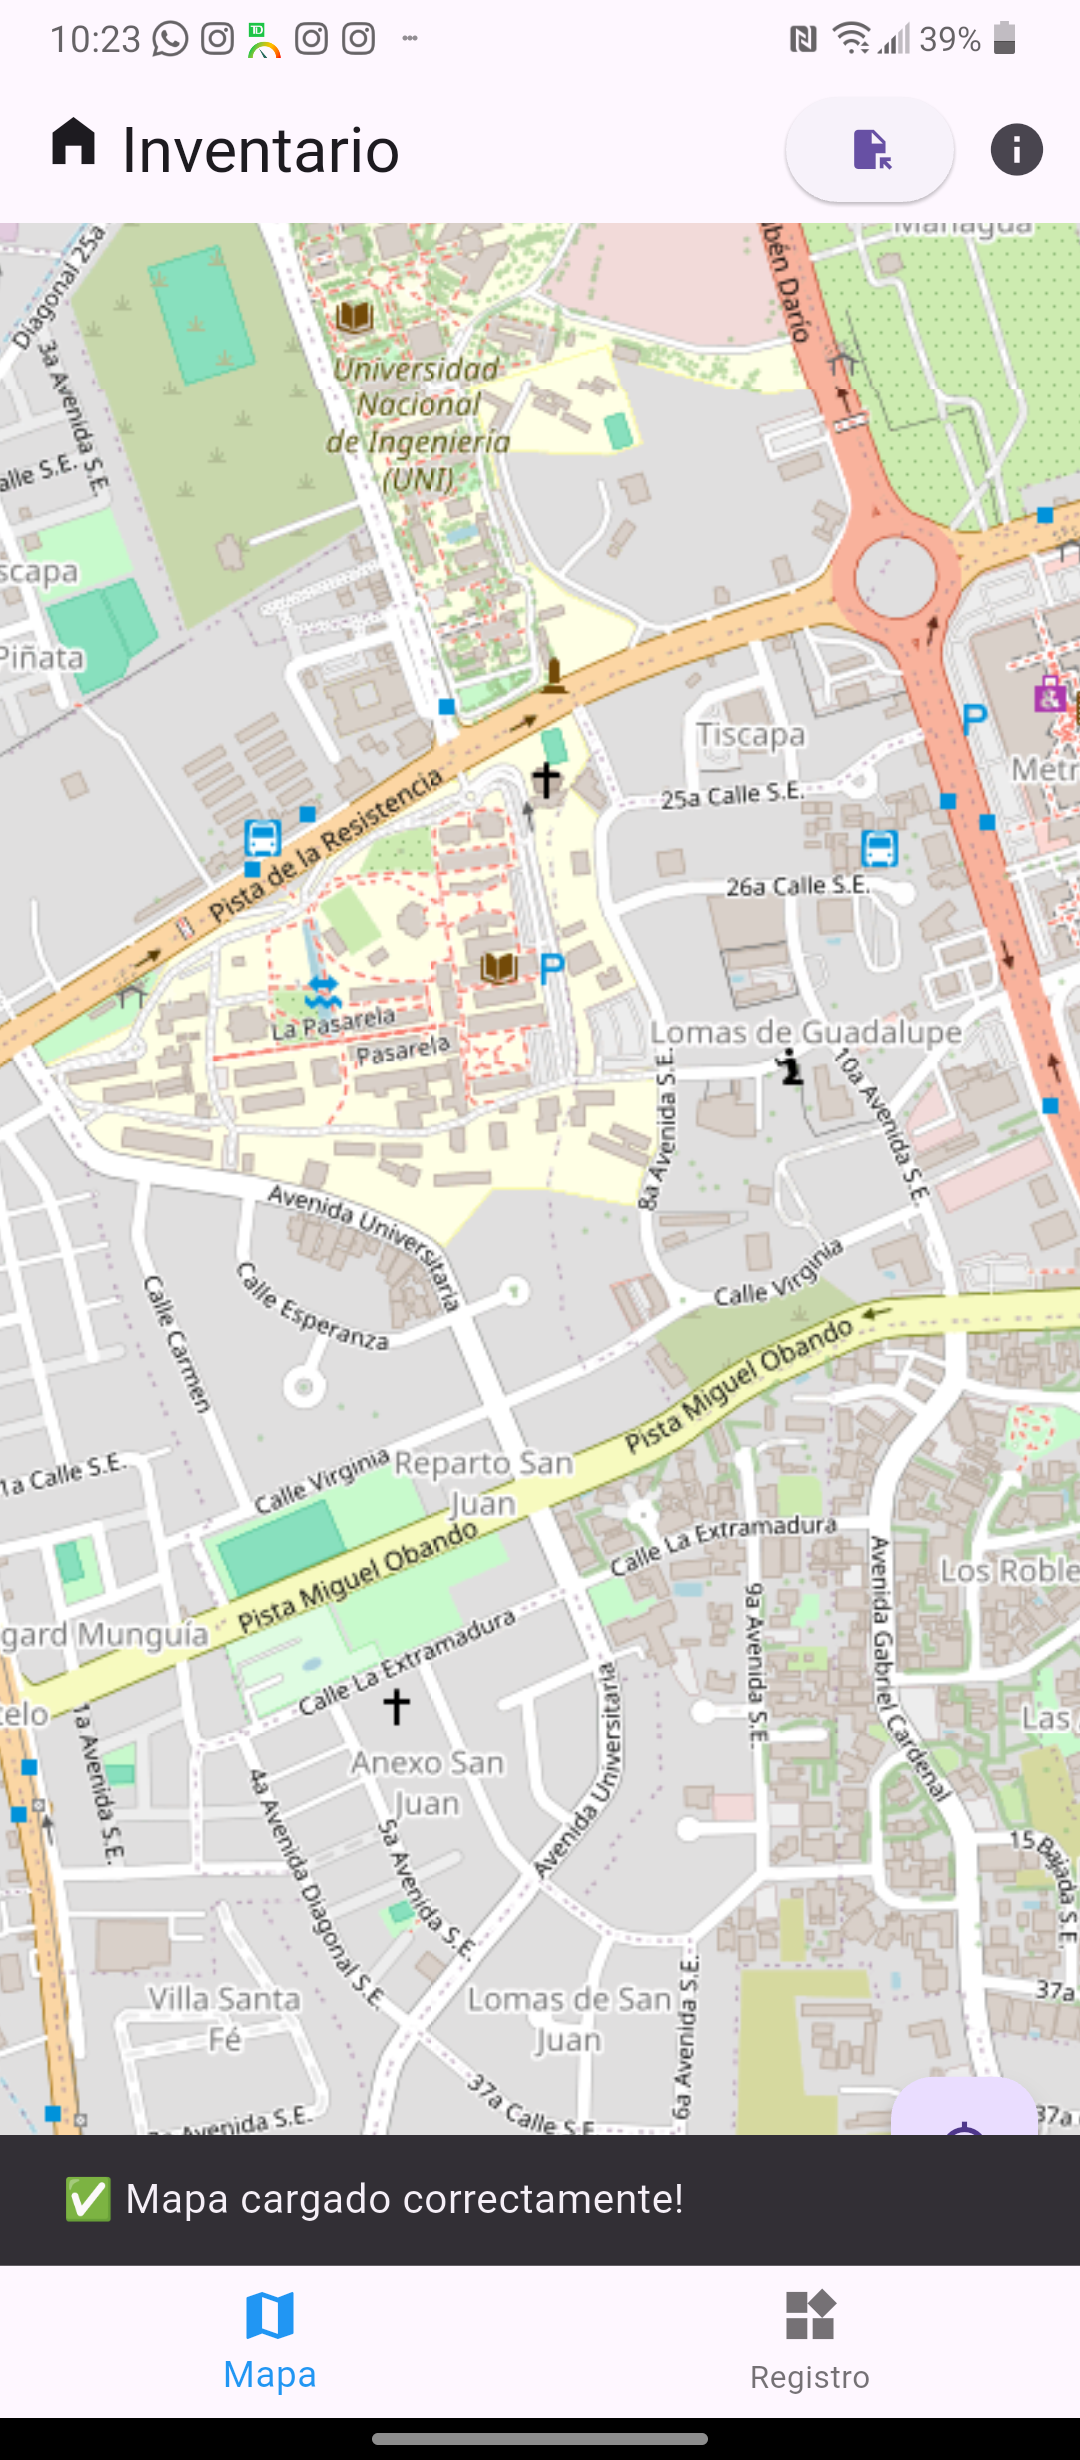
\includegraphics[width=0.3\textwidth]{Graphics/Capitulo 4/LG Android 13/4.2/2.png}
    \caption{Prueba de importación de mapa}
    \label{fig:figura20}
\end{figure}
Esta constituye una prueba básica de las funcionalidades de la aplicación pero se debe tener en cuenta que también se está analizando compatibilidad
con versiones de Android antiguas como la 10 y esto es una prueba válida dada la inmensa cantidad de variaciones que se han creado desde 2019(seis años atrás)
hasta la actualidad en actualizaciones del SO.

\pagebreak
\section{Importación de varias capas de delimitación, una de ellas con el formato de predios}
Esta acción, al igual que la importación de un mapa, puede llevarse a cabo de manera manual o mediante el botón con esta funcionalidad ubicado en la ventana
que se muestra al presionar el botón con icono de archivo en la esquina superior derecha de la aplicación. Para hacerlo de manera
manual, se colocan todas las delimitaciones como archivos con extensión '.geojson' que se desean mostrar sobre el mapa, en la carpeta "$ $CADIC/Delimitaciones"$ $
ubicada en el directorio raíz del dispositivo. Los resultados se aprecian en la figura \ref{fig:figura21}
\begin{figure}[h]
    % \centering
    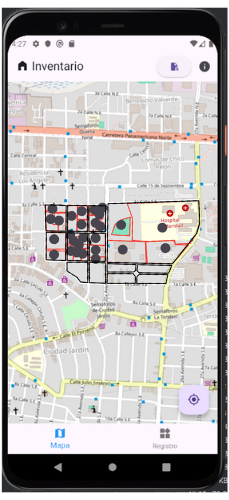
\includegraphics[width=0.3\textwidth]{Graphics/Capitulo 4/Pixel 4 [emulador]/4.3/1.png}
    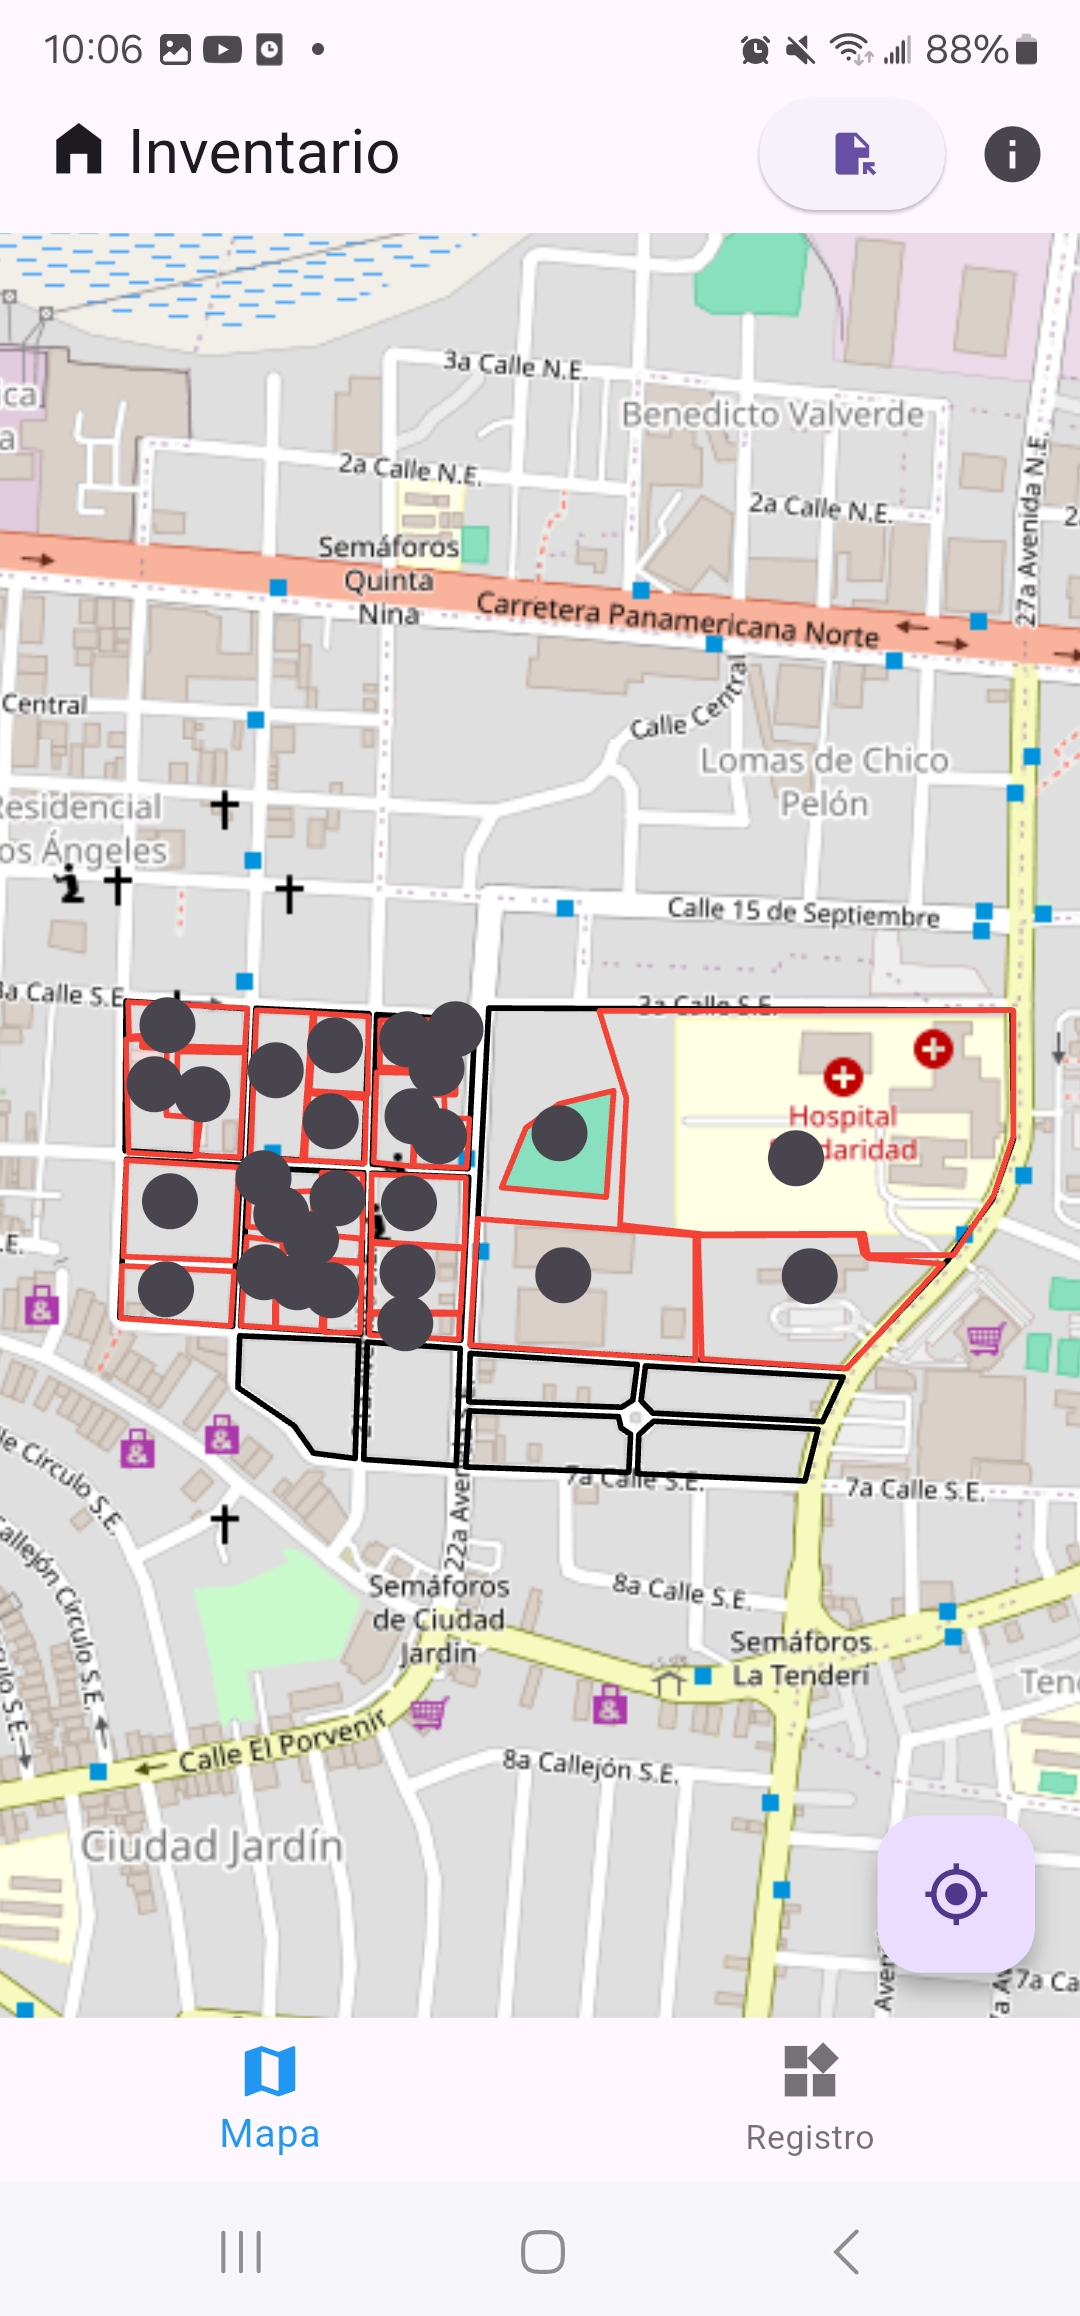
\includegraphics[width=0.3\textwidth]{Graphics/Capitulo 4/Galaxy S23 Ultra Android/4.3/4.jpg}
    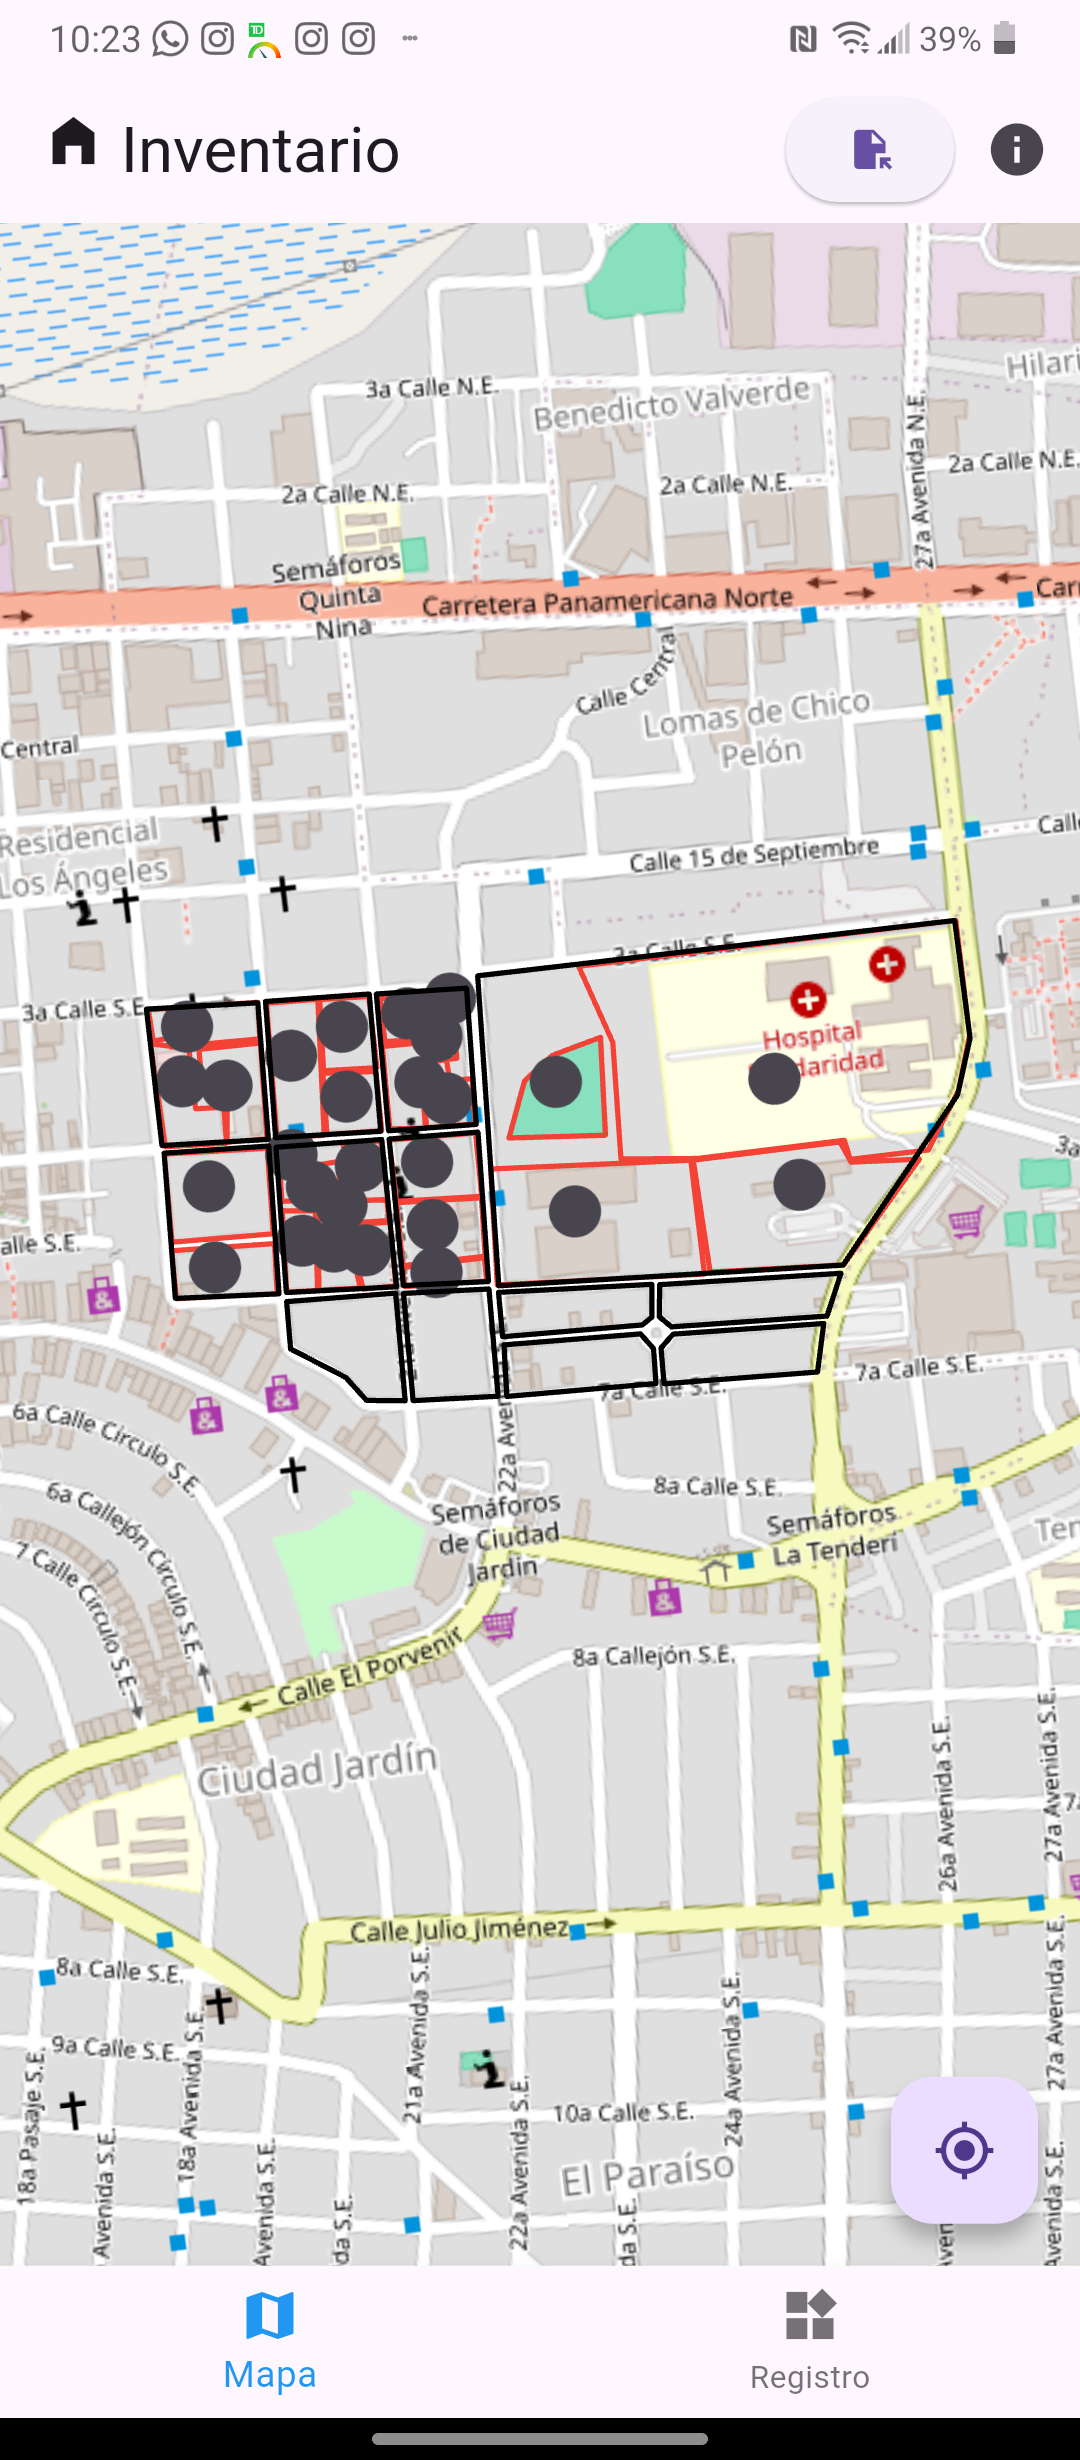
\includegraphics[width=0.3\textwidth]{Graphics/Capitulo 4/LG Android 13/4.3/1.png}
    \caption{Prueba de importación de capa de delimitaciones}
    \label{fig:figura21}
\end{figure}
Se probó la funcionalidad de importación de mapa y ahora de delimitaciones y resultó sin problemas en las tres versiones diferentes de Android. Hay que decir que tanto esta funcionalidad
como la de importar mapa, son no imprescindibles, ya que al abrirse la aplicación por primera vez, esta crea el directorio CADIC en la raíz del almacenamiento
del dispositivo, y dentro tres subdirectorios donde se pueden copiar las delimitaciones o el mapa y estos cargarán igualmente bien.

\pagebreak
\section{Validación de Formularios}
Esta prueba se realiza sobre la funcionalidad principal de la aplicación, la introducción de datos y validación de los formularios. La sección de formularios se encuentra en la
pestaña 'Registro', y aquí se rellena e introduce toda la información de los predios, edificios y propiedades en la base de datos de la aplicación. Al rellenar los campos obligatorios
de un subformulario y presionar en el botón "Guardar"$ $ del mismo, se validará la información introducida. En caso de que falten campos por rellenar, o que los datos no estén correctos en
una o más entradas, los campos con problema se mostrarán resaltados con letras rojas y no se guardarán los datos. En caso de que todo esté correctamente rellenado, la aplicación procede a
guardar los datos en la base de datos local, mostrando un mensaje en una barra emergente que diría "$ $Datos guardados"$ $. Resultados provenientes de diferentes escenarios en los que se introducen
datos correctos, incorrectos o incompletos se observan en la figura \ref{fig:figura22}.
\begin{figure}[h]
    % \centering
    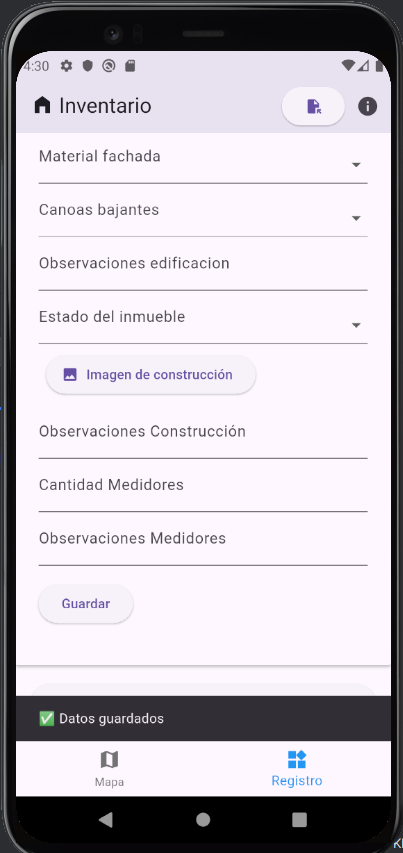
\includegraphics[width=0.3\textwidth]{Graphics/Capitulo 4/Pixel 4 [emulador]/4.4/1.png}
    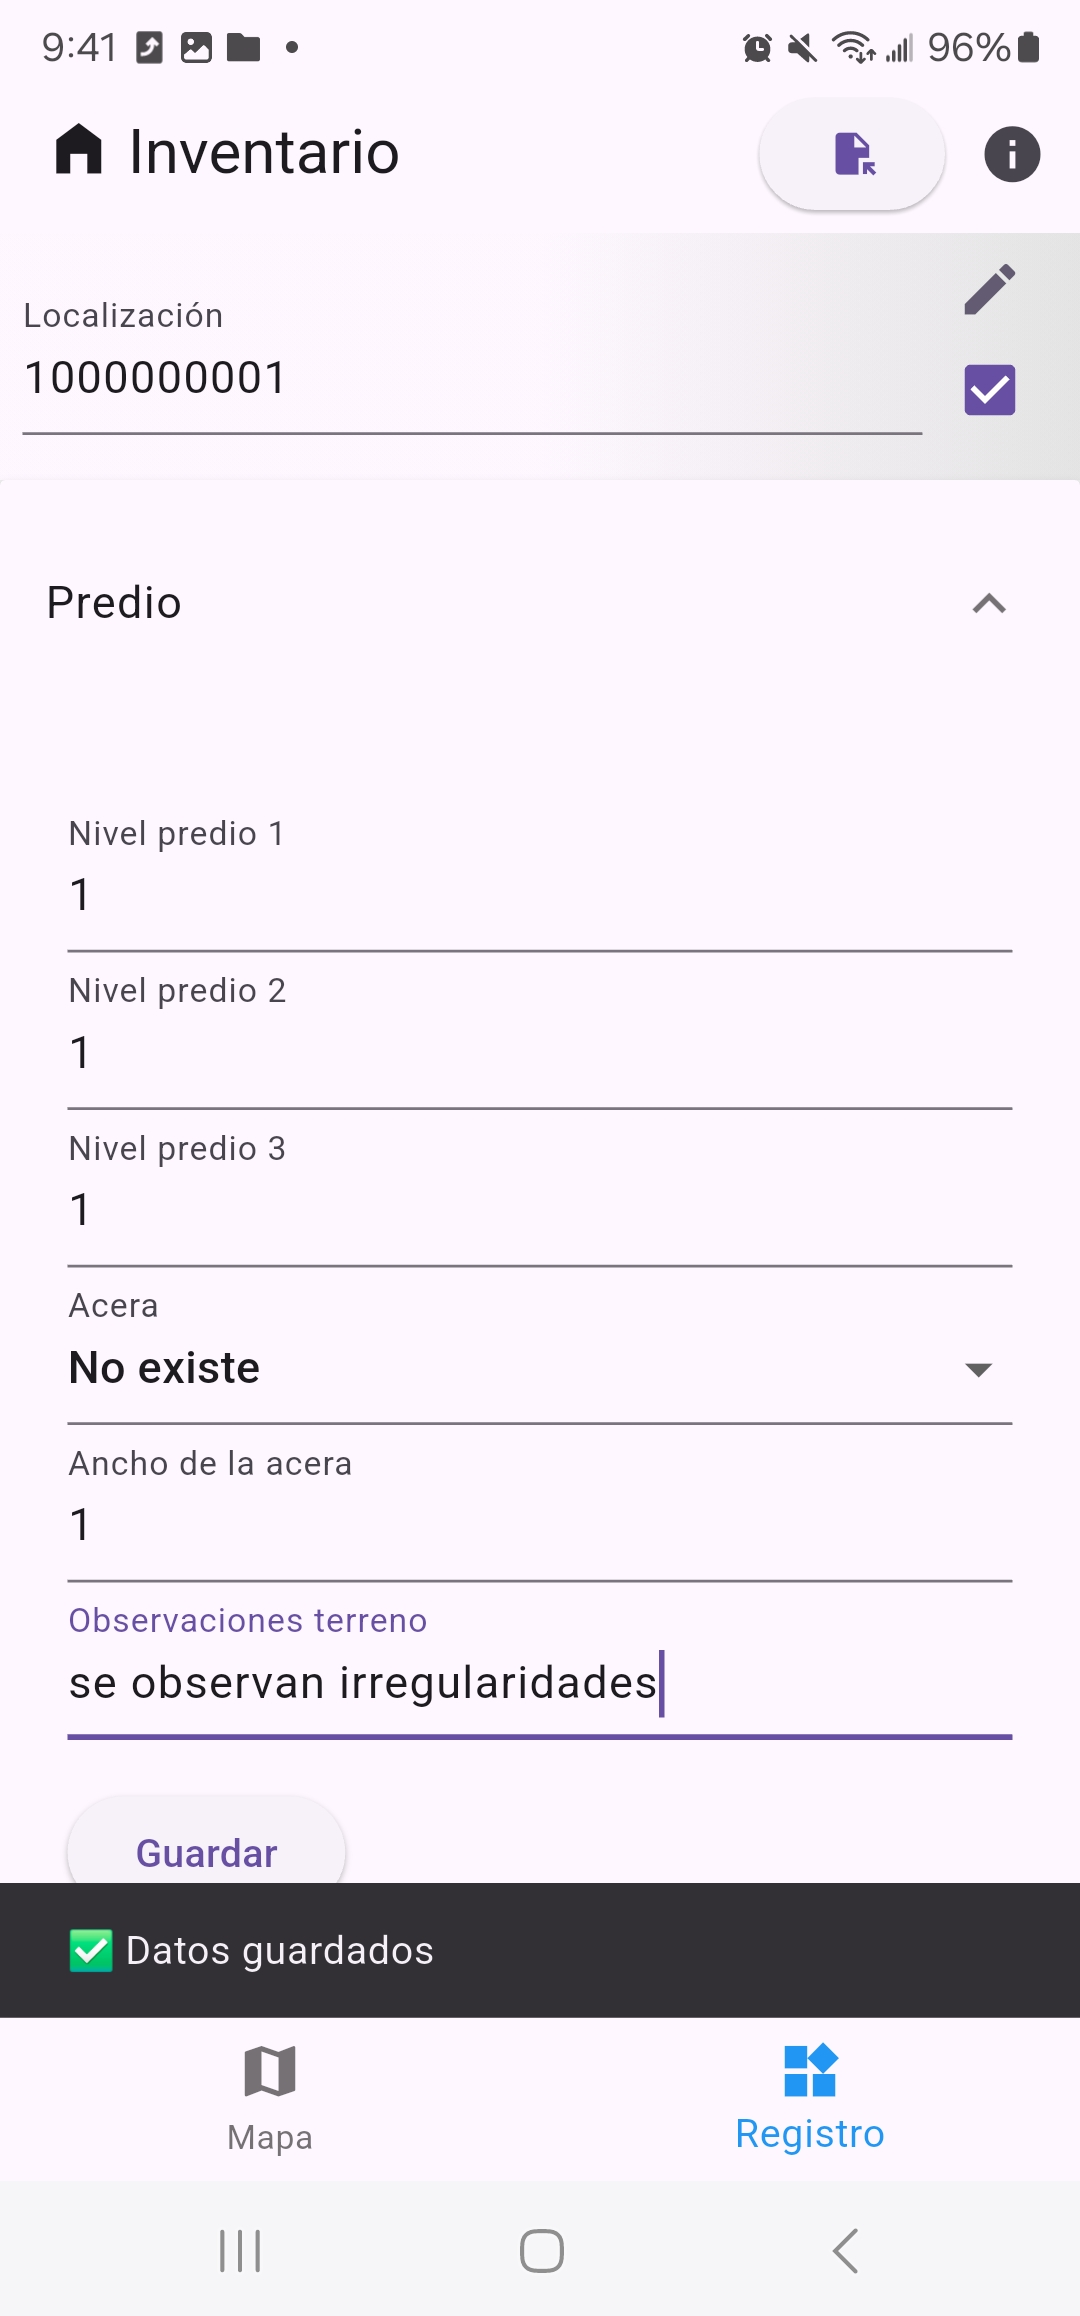
\includegraphics[width=0.3\textwidth]{Graphics/Capitulo 4/Galaxy S23 Ultra Android/4.4/1.jpg}
    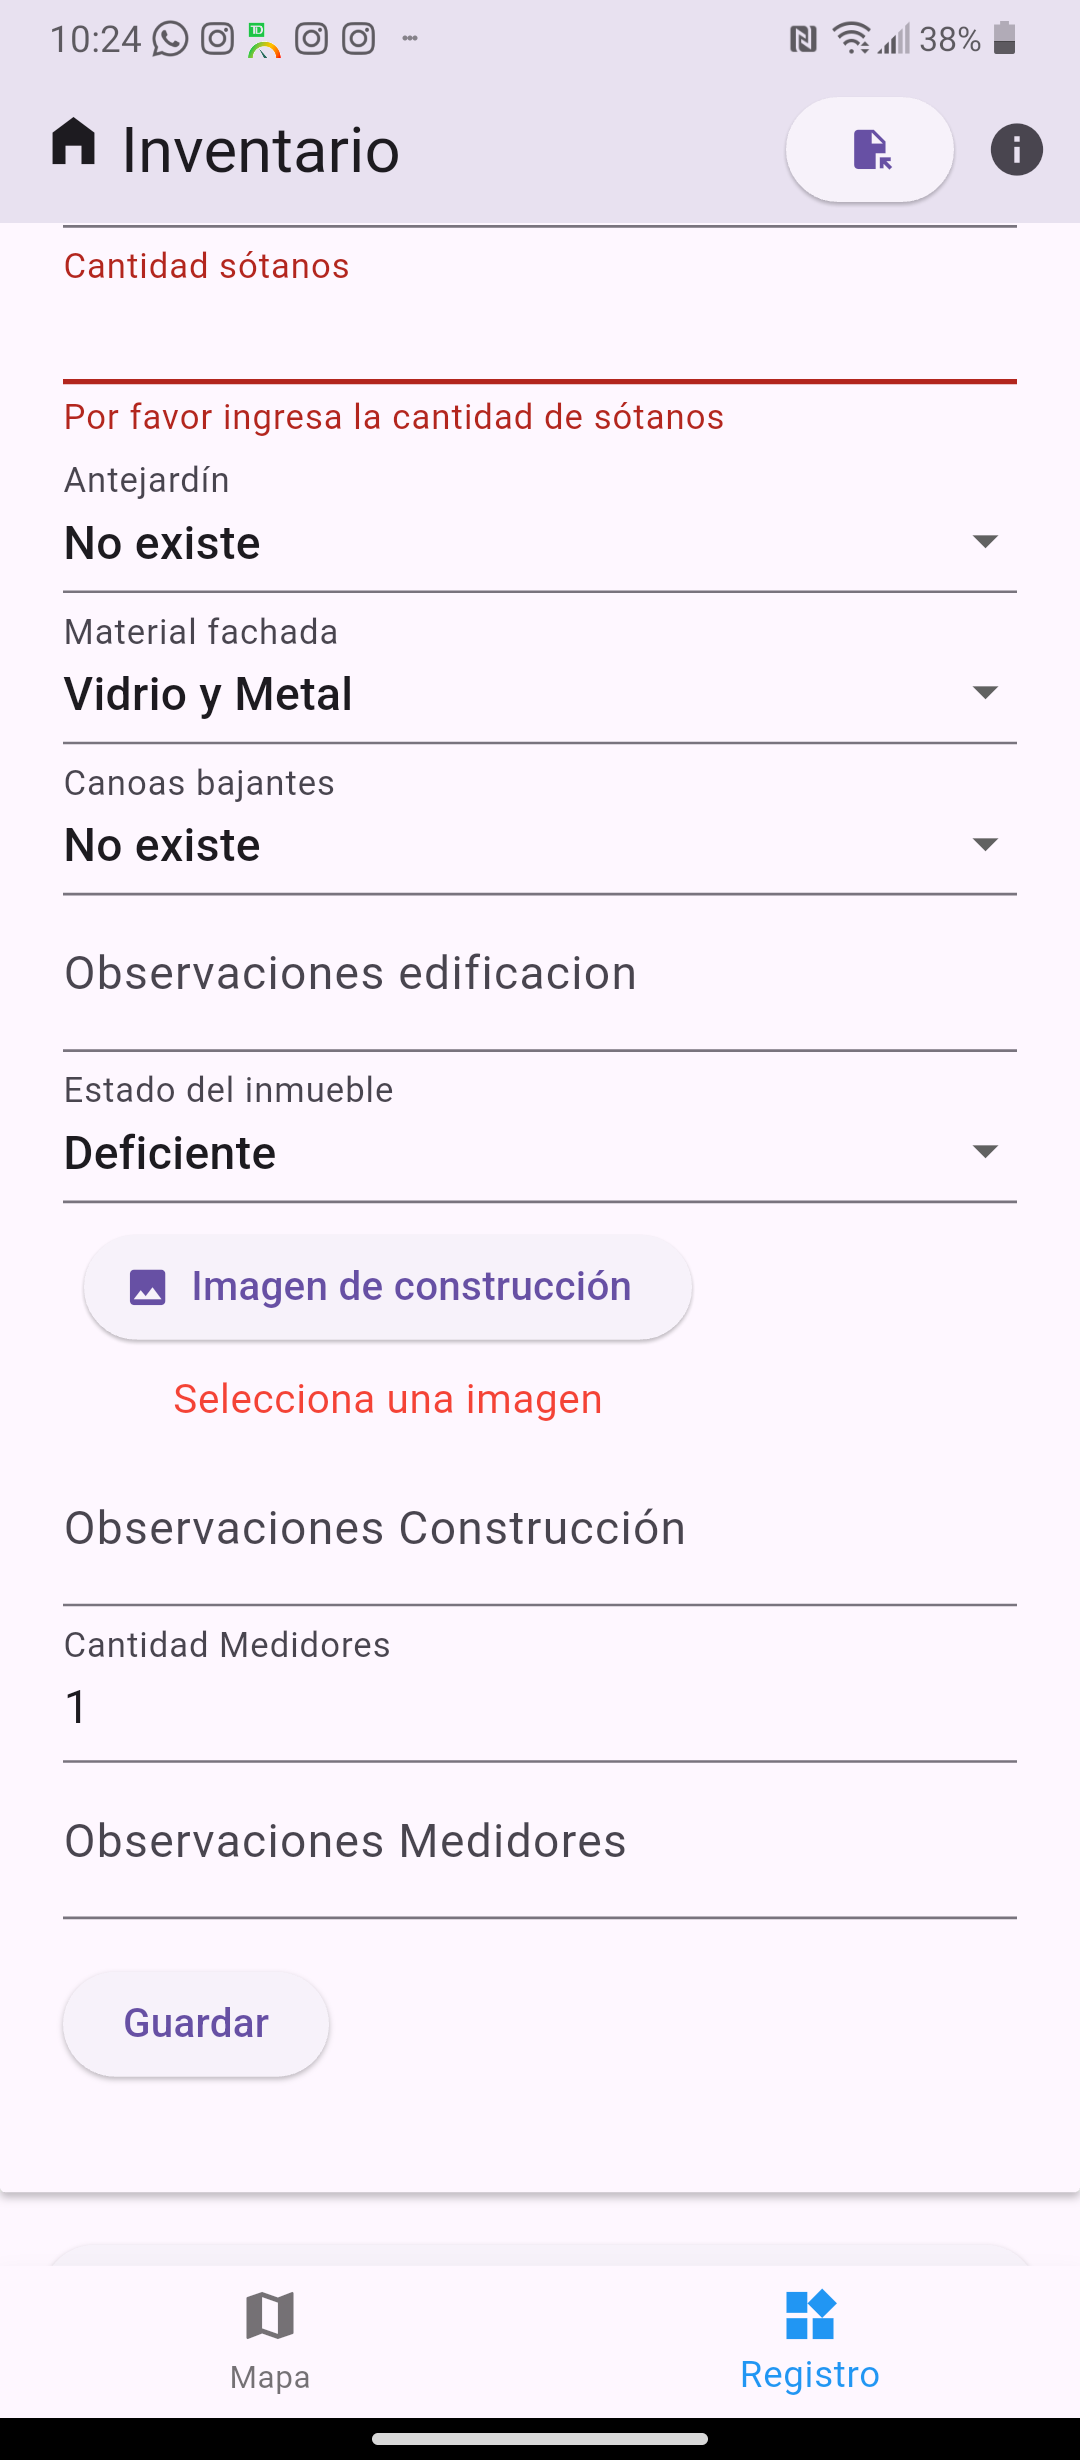
\includegraphics[width=0.3\textwidth]{Graphics/Capitulo 4/LG Android 13/4.4/2.png}
    \caption{Prueba de validación de formularios}
    \label{fig:figura22}
\end{figure}

Los campos que se marcaron en rojo no se rellenaron a propósito con el objetivo de mostrar que la
validación funciona. La aplicación sigue teniendo el comportamiento esperado en las tres versiones de Android.

\pagebreak
\section{Edición, recuperación y eliminación de Propiedades y Edificios}
La Edición, recuperación y eliminación de datos también es otra parte fundamental de la aplicación. De manera general, al introducir e intentar guardar datos en
los diferentes subformularios, estos actuarán de manera reactiva a los nuevos datos, mostrando información ya presente en la base de datos, e incluyendo los nuevos datos que
se introdujeron. En caso de estar sobrescribiendo los datos, ya sea de un predio, un edificio o una propiedad se advierte al usuario lanzando mensajes de error o de precaución.
Estos mensajes también se lanzan en casos específicos como al asociar un edificio ya registrado a un predio diferente. Para editar un edificio o propiedad se debe presionar
en el elemento visual que representa este elemento en la lista de edificios asociados al predio actual seleccionado o en la lista de propiedades asociadas al edificio actual
seleccionado (para más detalle, ver apartado del epígrafe \ref{section:casosDeUso}).
\begin{figure}[h]
    % \centering
    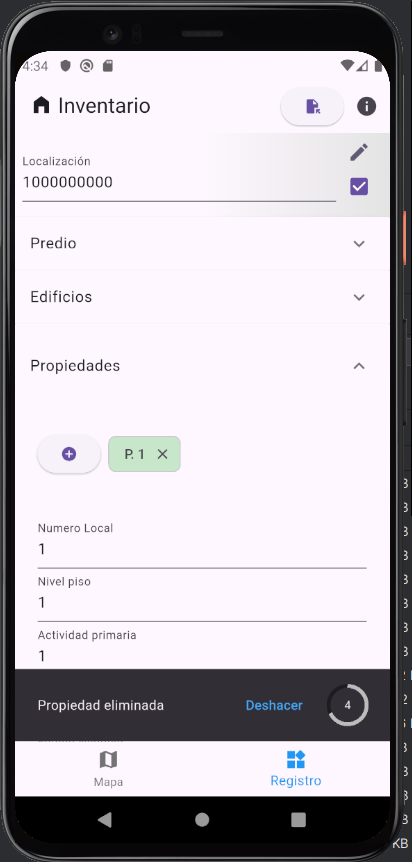
\includegraphics[width=0.3\textwidth]{Graphics/Capitulo 4/Pixel 4 [emulador]/4.5/5.png}
    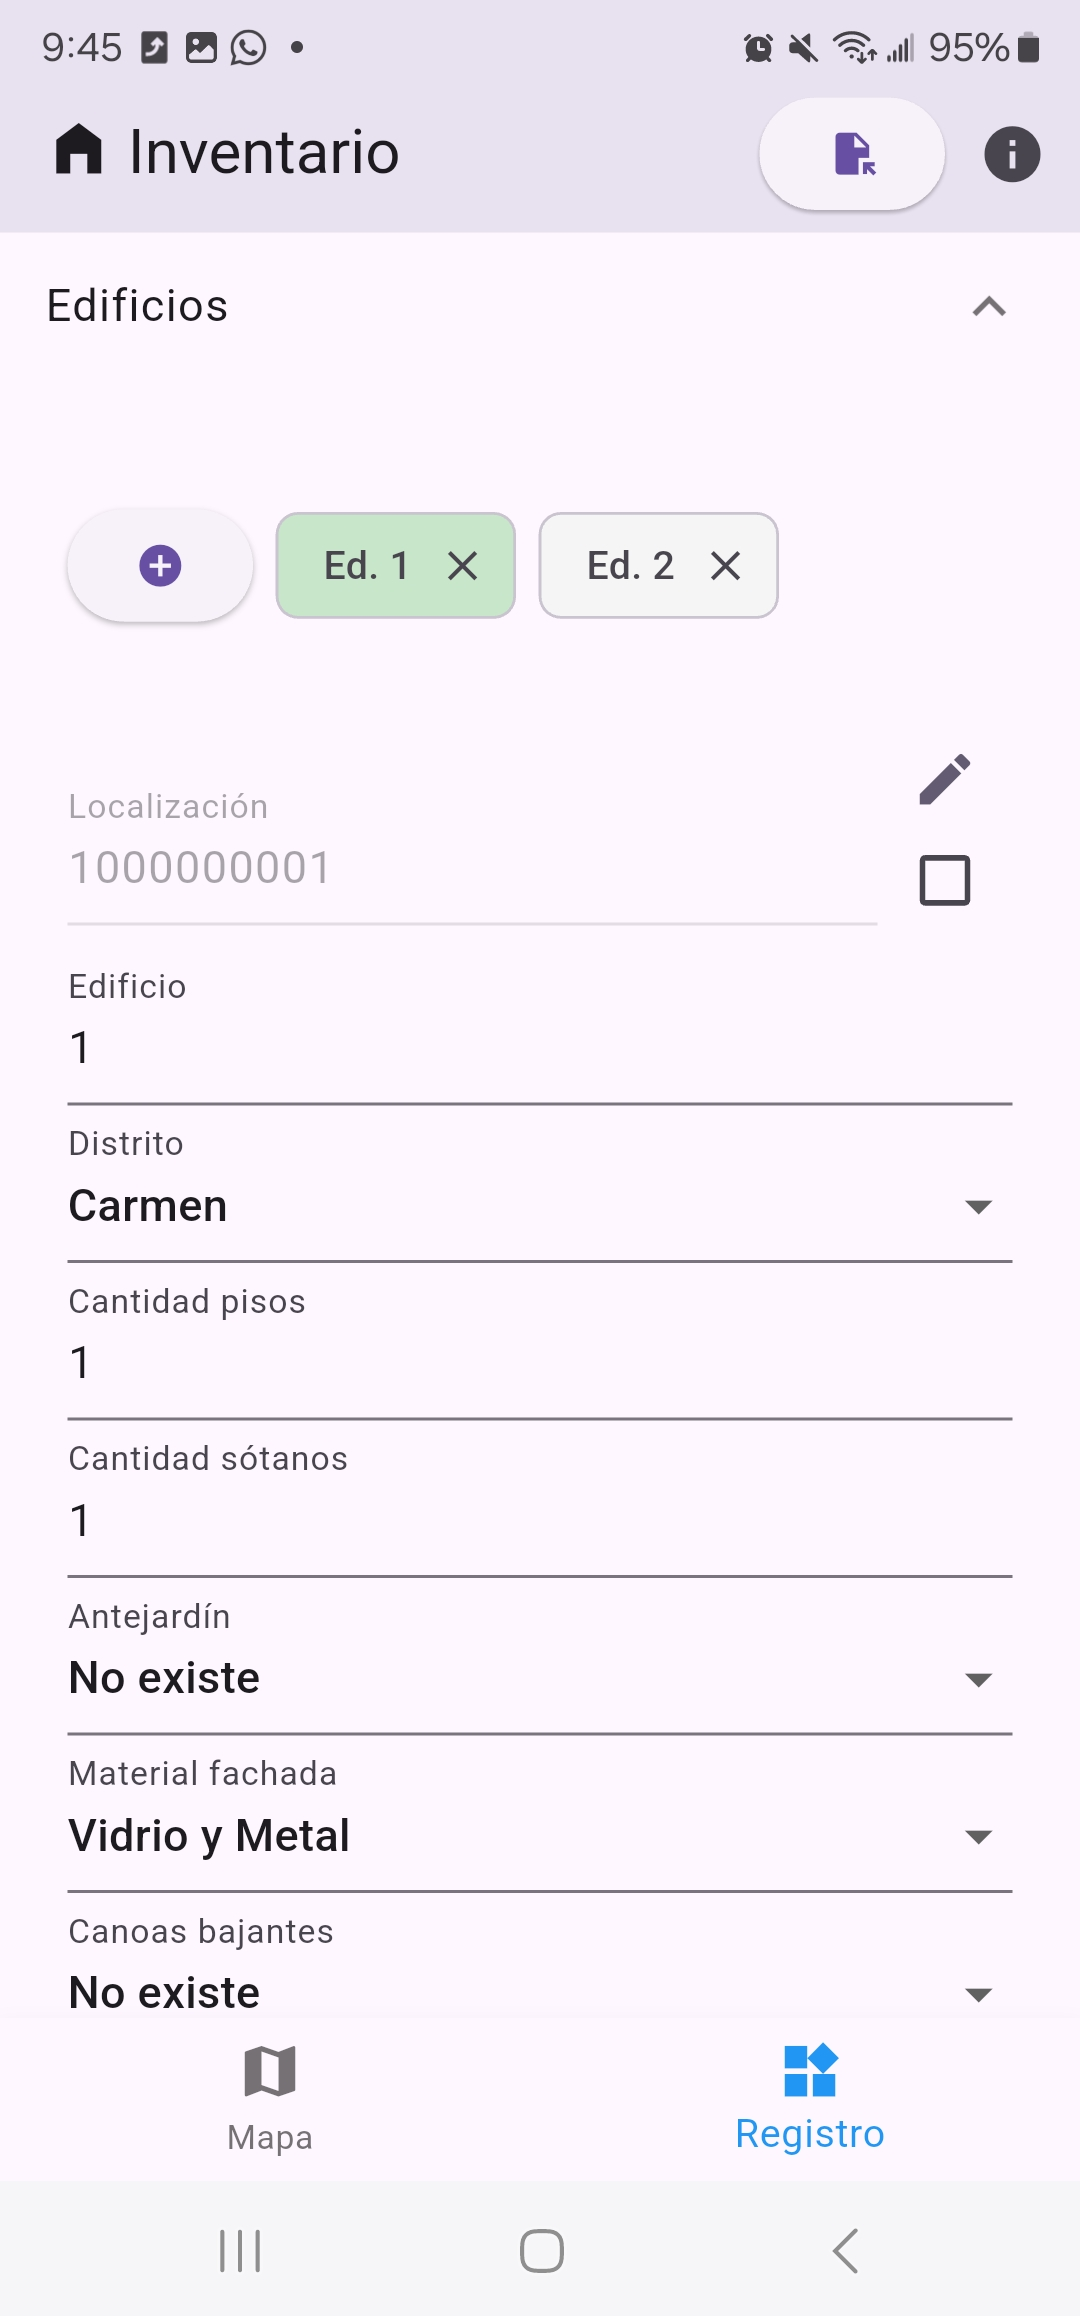
\includegraphics[width=0.3\textwidth]{Graphics/Capitulo 4/Galaxy S23 Ultra Android/4.5/1.jpg}
    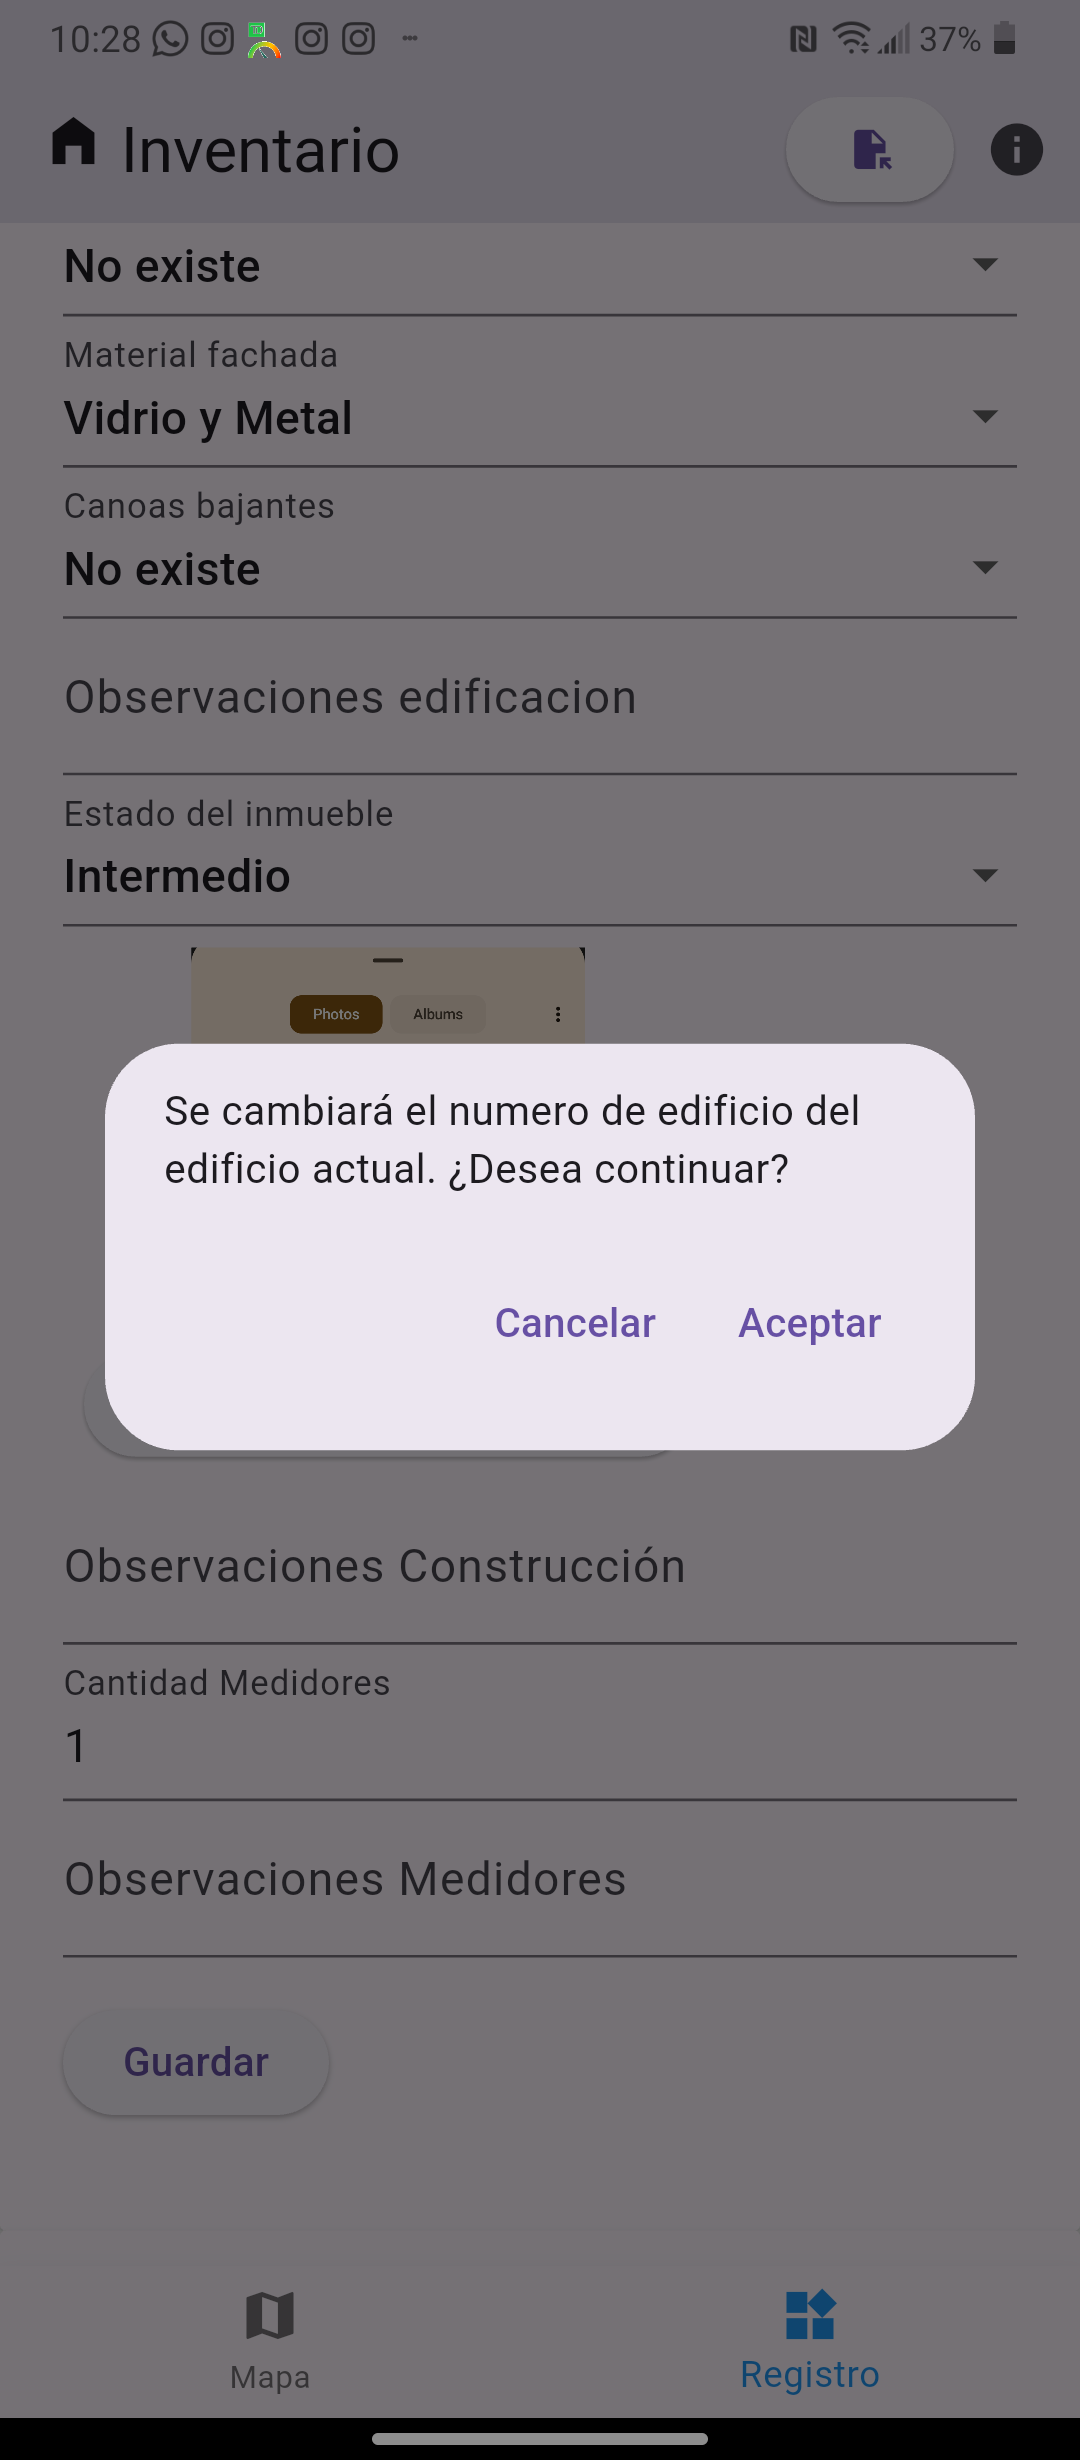
\includegraphics[width=0.3\textwidth]{Graphics/Capitulo 4/LG Android 13/4.4/4.png}
    \caption{Prueba de edición, recuperación y eliminación de Edificios y propiedades}
    \label{fig:figura23}
\end{figure}

En la figura \ref{fig:figura23} se aprecian varios escenarios de edición, eliminación y recuperación de datos de propiedades y edificios. En la imagen de la extrema derecha
se observa un mensaje de confirmación ya que se optó por cambiar el número de edificio de un edificio existente, lo cual es una acción poco usual y por ende se agrega un paso de confirmación.
En la imagen de la izquierda, podemos apreciar la eliminación de una entidad. Ya sea Edificio o Propiedad, al eliminar alguna entidad, se eliminará al final de un contador que da la oportunidad
de deshacer la eliminación. Las respuestas a la actual pueba fueron satisfactorias para todas las versiones de Android.


\section{Marcando varios predios como visitados}
Una funcionalidad no tan primordial, pero sin embargo bastante útil, es la de marcar los predios ya visitados por el encuestador que opera la aplicación, esto se realiza de manera sencilla en
la pestaña 'Registro'(para m'as detalle, ver apartado del epígrafe \ref{section:casosDeUso}). En esta prueba se testea dicha funcionalidad, buscando que los predios marcados como visitados, estén
marcados en el mapa en color verde, mientras que los que no se hayan marcado aún permanezcan con bordes rojos.
\begin{figure}[h]
    \centering
    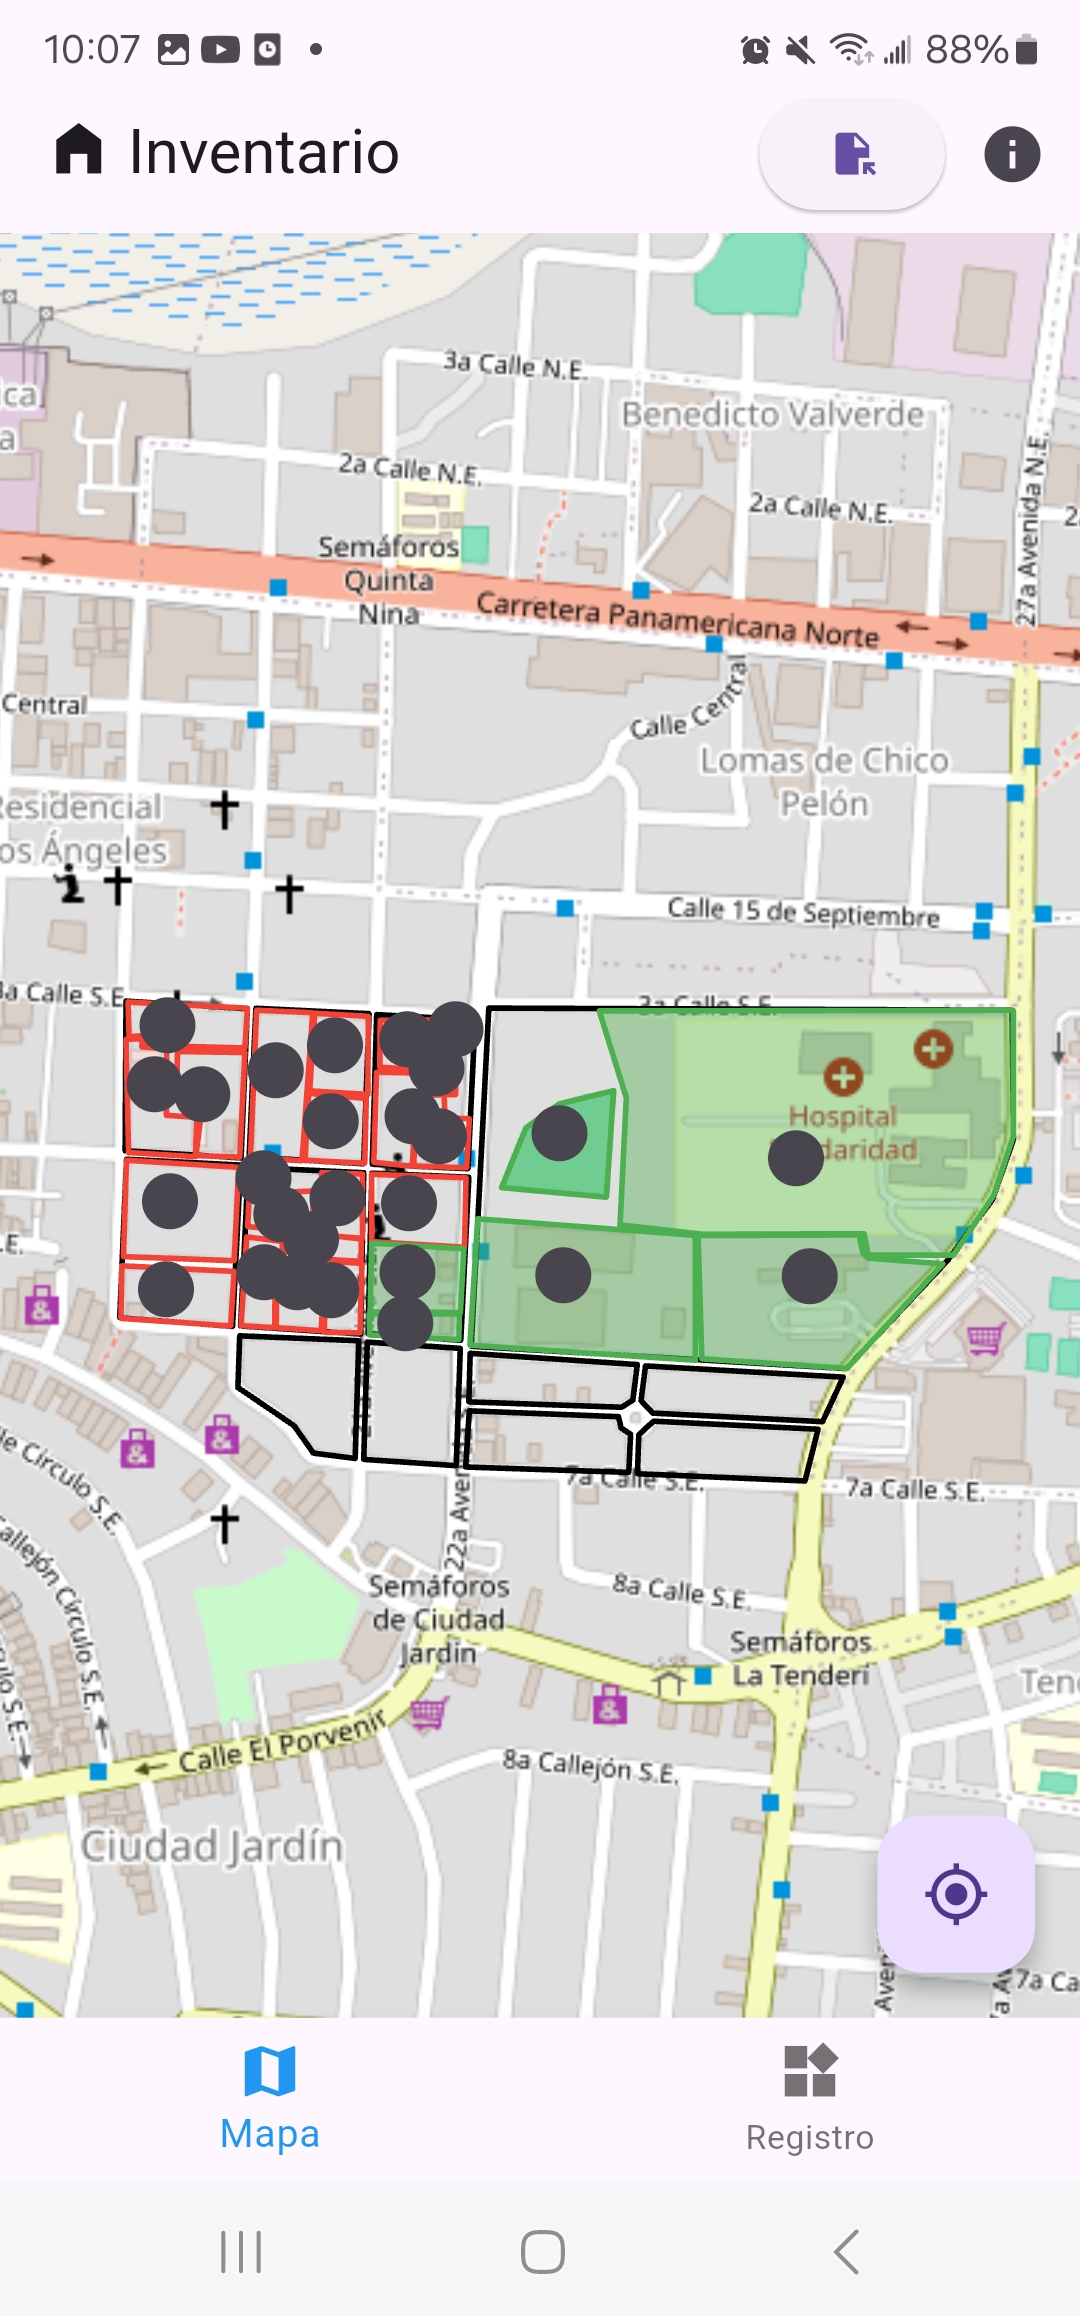
\includegraphics[width=0.3\textwidth]{Graphics/Capitulo 4/Galaxy S23 Ultra Android/4.6/1.jpg}
    \caption{Prueba de la funcionalidad de marcar predios como visitados}
    \label{fig:figura24}
\end{figure}
En la figura \ref{fig:figura24} se puede observa el resultado de la prueba, satisfactoriamente pasada.
\pagebreak
\section{Exportación y Limpieza de la Base de Datos}
Esta última prueba se hace sobre dos funcionalidades que son consideradas en conjunto como la vía de conexión de la aplicación con la entidad centralizada que reúne la información recogida
por todos los encuestadores, en un solo sitio. Se usa la funcionalidad de exportar la base de datos, se comprueba con un programa de terceros(SQLite Viewer \cite{sqliteViewer}) que esta contiene los datos insertados manualmente
en la aplicación y luego se pasa a limpiar la base de datos.
\begin{figure}[h]
    \centering
    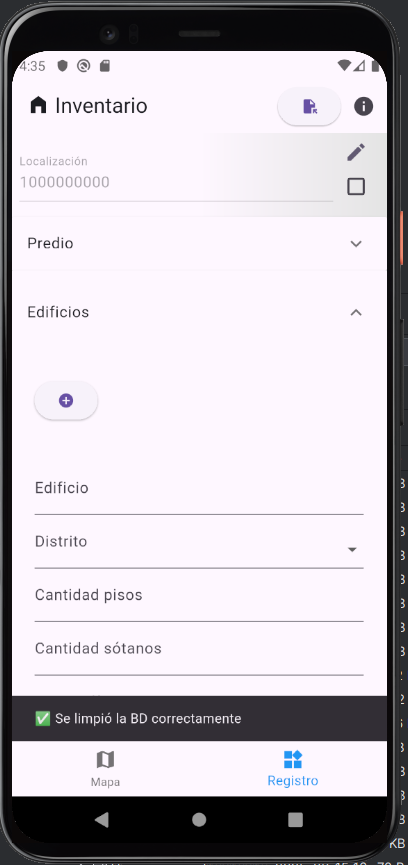
\includegraphics[width=0.3\textwidth]{Graphics/Capitulo 4/Pixel 4 [emulador]/4.7/1.png}
    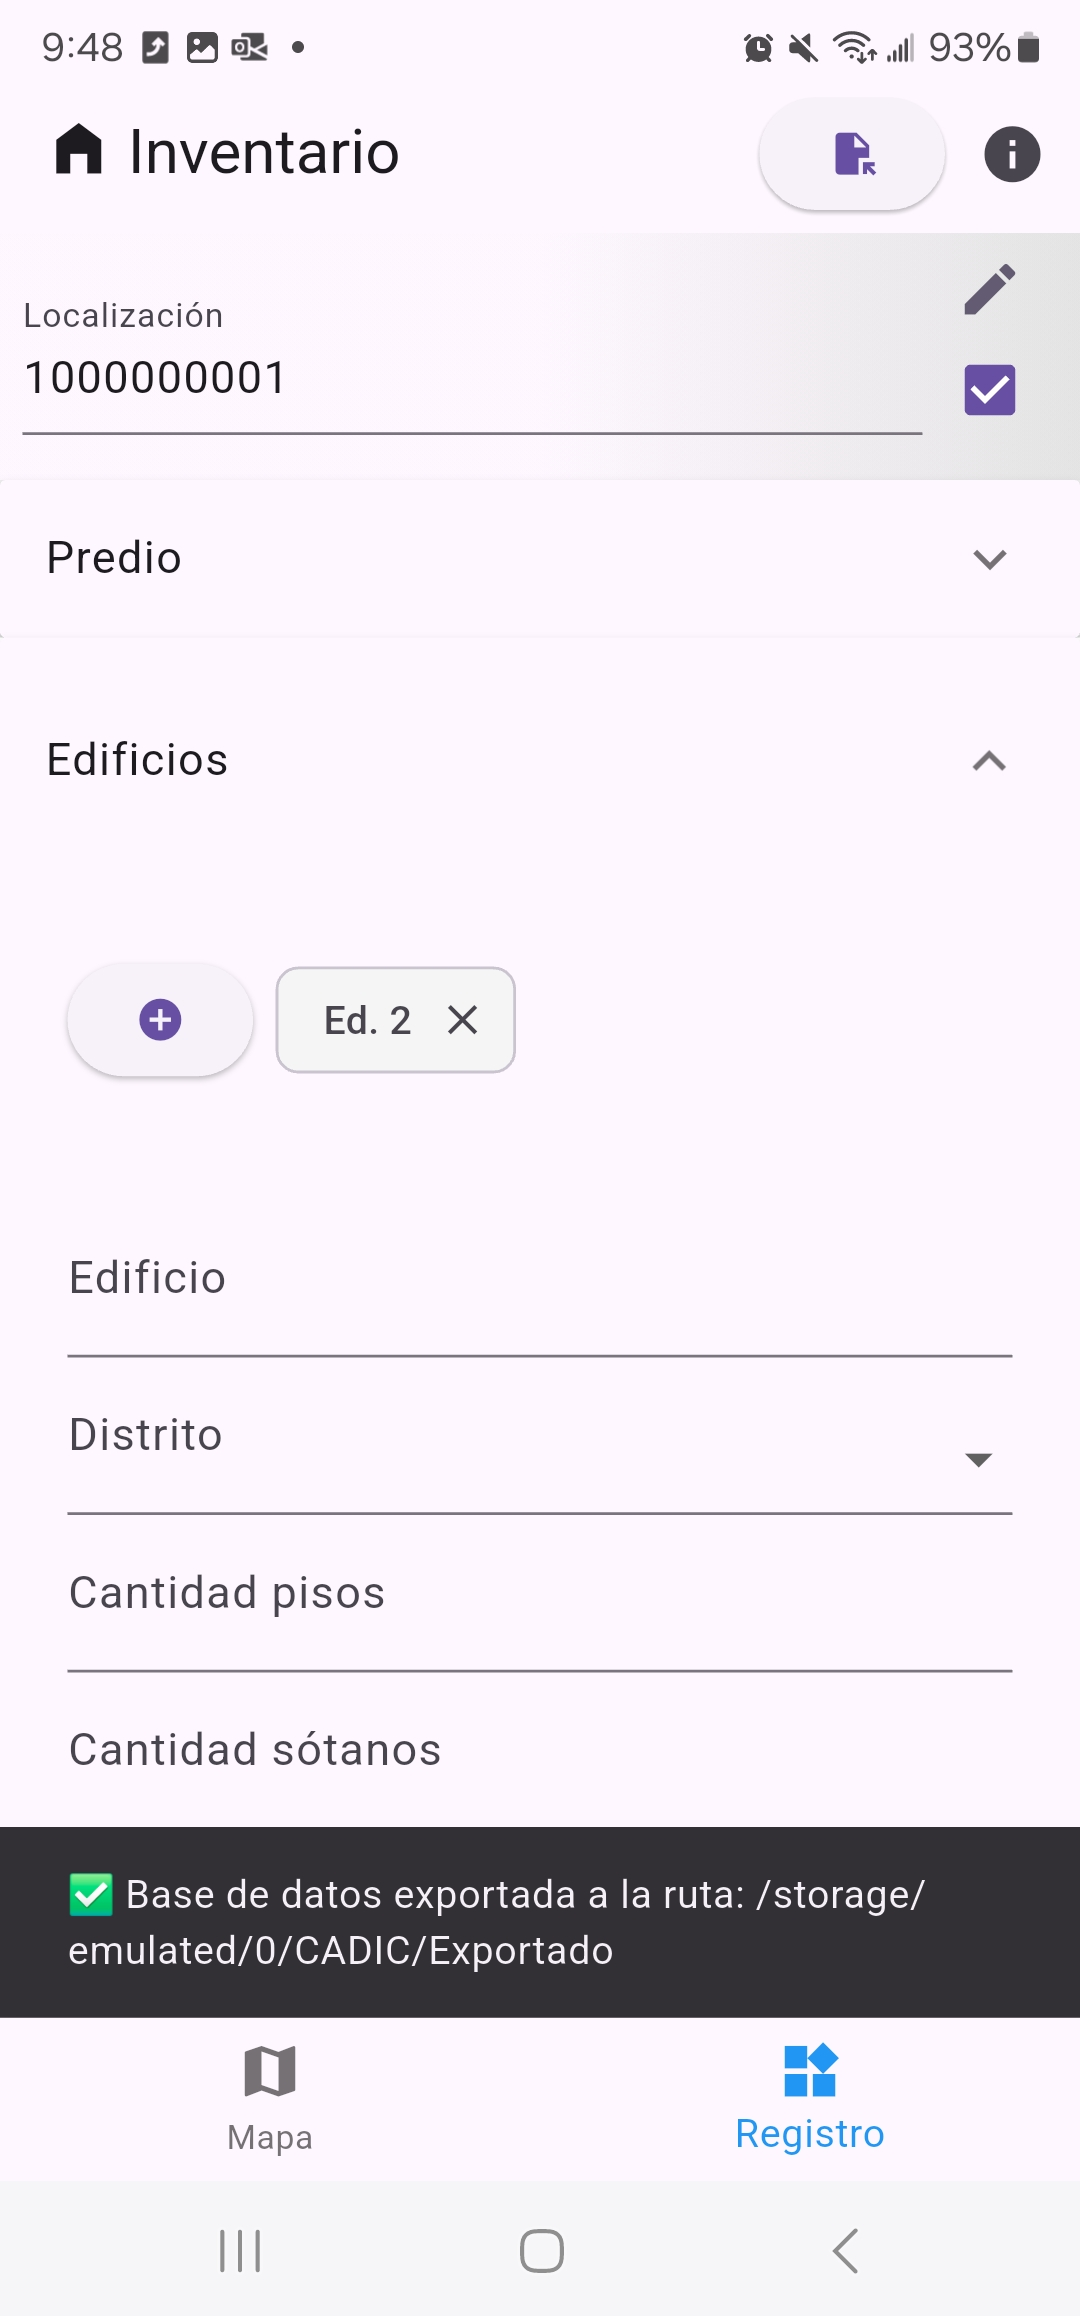
\includegraphics[width=0.3\textwidth]{Graphics/Capitulo 4/Galaxy S23 Ultra Android/4.7/1.jpg}
    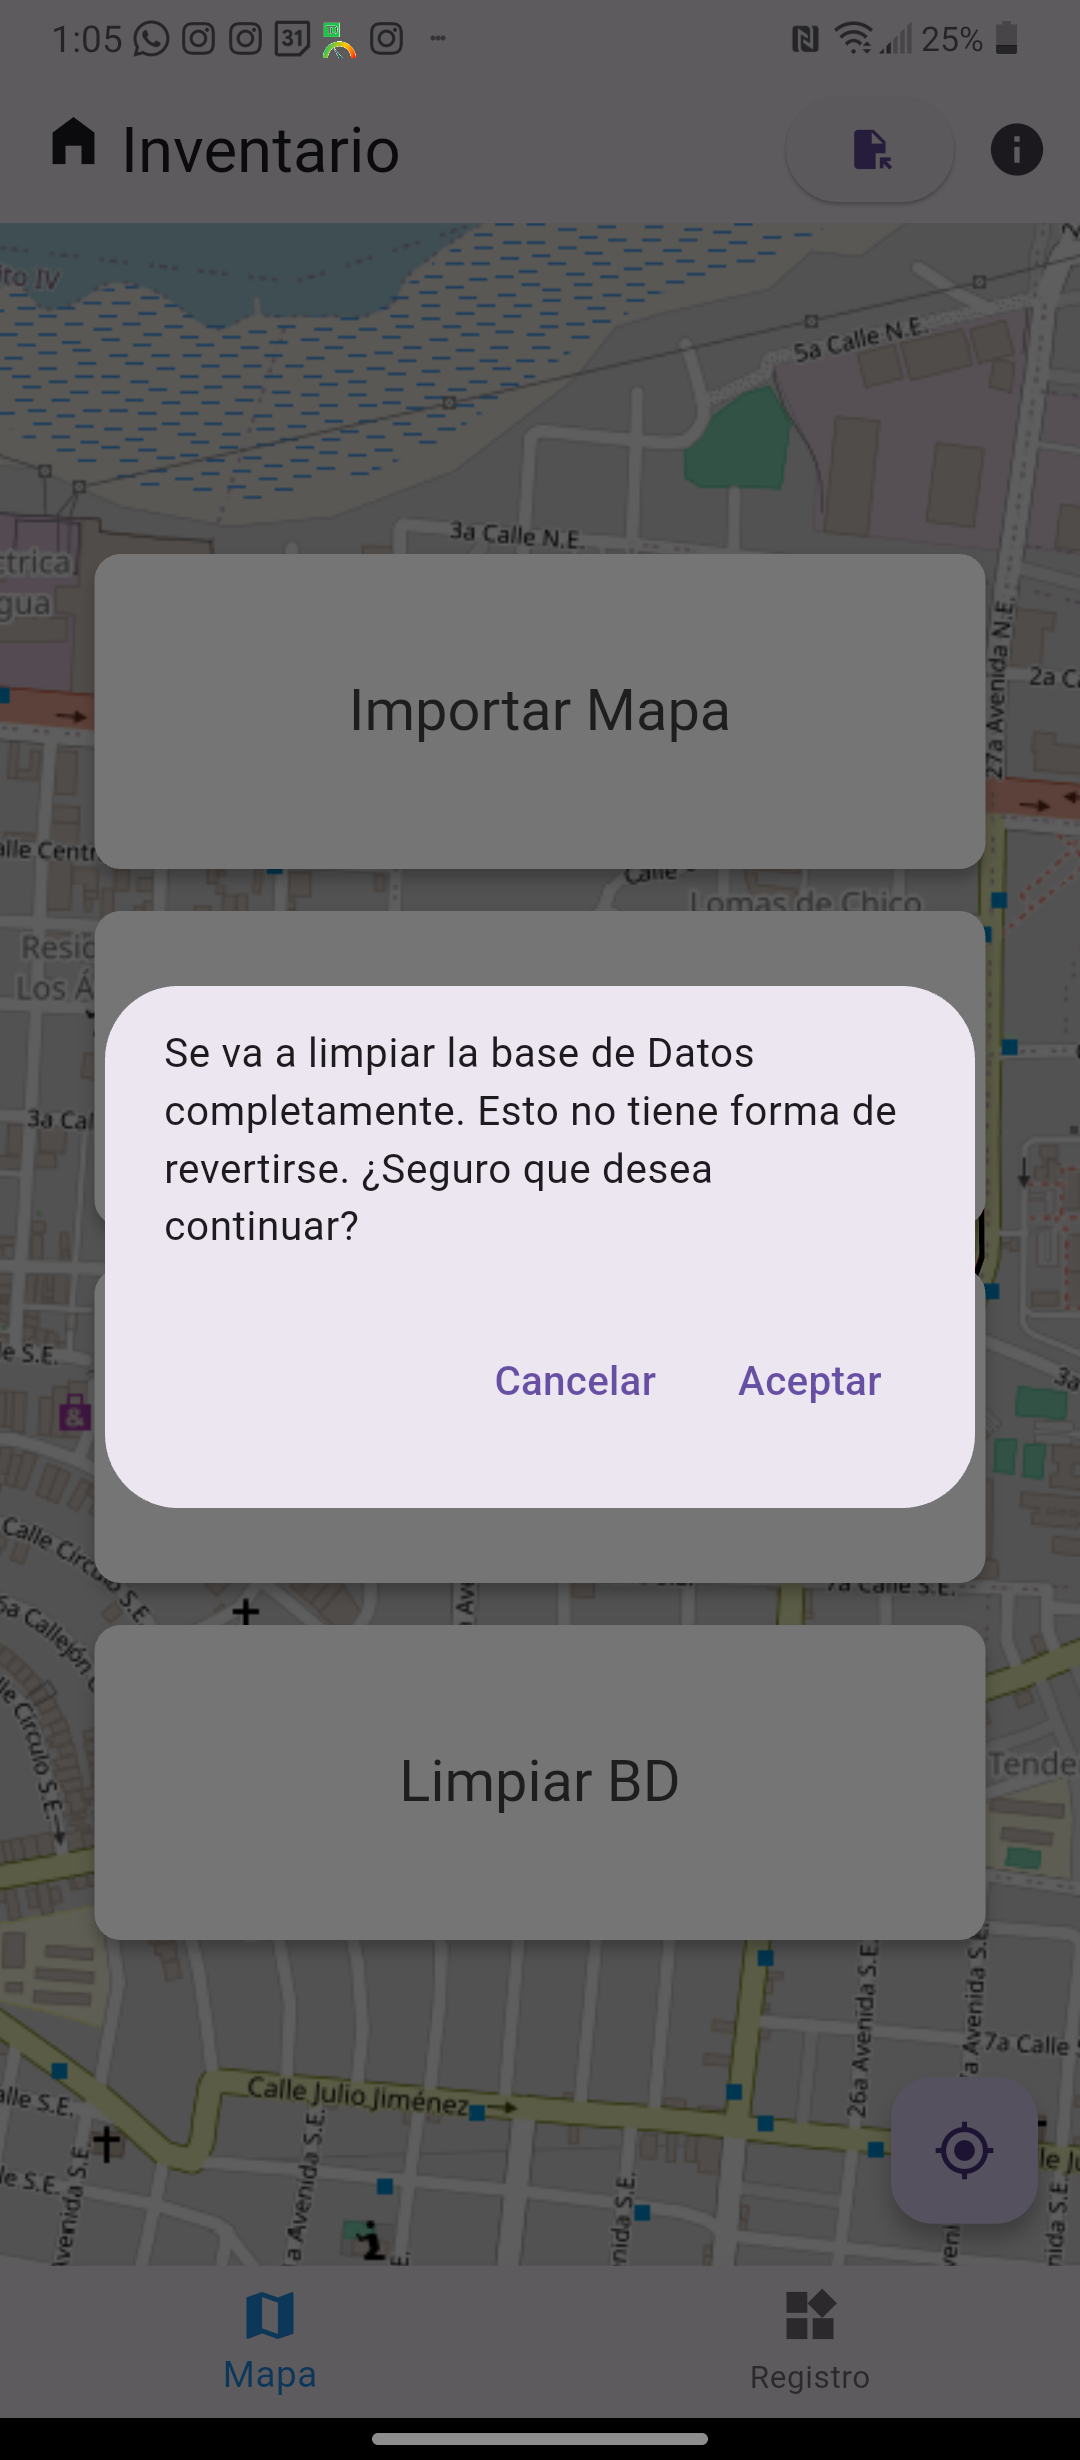
\includegraphics[width=0.3\textwidth]{Graphics/Capitulo 4/LG Android 13/4.7/Screenshot_20250615-130550.png}
    \caption{Prueba de la funcionalidad de marcar predios como visitados}
    \label{fig:figura25}
\end{figure}
\begin{figure}[h]
    \centering
    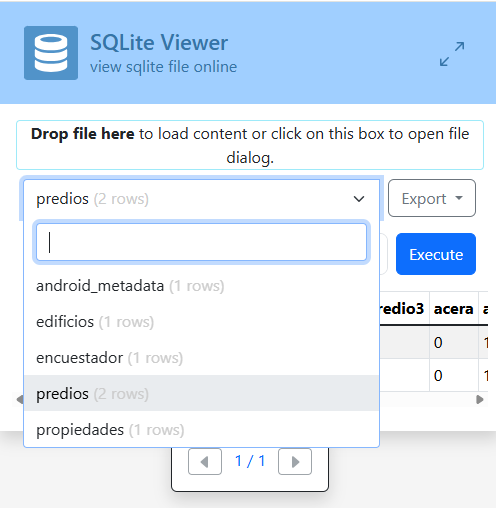
\includegraphics[]{Graphics/Capitulo 4/verificacion_BD_exportada.png}
    \caption{Verificación de consistencia de la base de datos luego de ser exportada.}
    \label{fig:figura26}
\end{figure}\\
Se realizó esta prueba con resultado satisfactorio, habiendo chequeando la consistencia de la base de datos luego de exportarla (Ver figura \ref{fig:figura26})
Recalcar que siempre se exporta la base de datos a la misma ruta/directorio: 'CADIC/Exportado' y también importante recalcar que al limpiar la base de datos se eliminan todas las tablas
excepto la que guarda el nombre del encuestador que está usando la aplicación.
Con esta prueba se concluyen todas las pruebas, habiendo pasado todas con éxito.


